% !TeX root = ../SDonchezThesis.tex

\chapter{Related Work}\label{ch:relatedWork}
Although the introduction of FPGAs into a cloud based environment has been a recent development, there exists some body of research conducted on such systems, as well as their security. Furthermore, substantial research has been conducted into various aspects of the architecture that are not necessarily cloud specific, such as bitstream security and the integrity of the partial reconfiguration process itself. A brief survey of those efforts is provided below, culminating in a detailed analysis of the specific prior work which proposes the architecture this effort seeks to extend.

\section{Vulnerabilities of DPR-enabled FPGA devices} \label{sec:vulnerabilities}
Before embarking on an analysis of academic efforts to mitigate DPR-based vulnerabilities (such as would apply to multi-tenant cloud devices), it is helpful to consider the extent and nature of those vulnerabilities in the first place. \cite{duncan_fpga_2019} provides a comprehensive overview of the entire bitstream security process from generation to transfer to loading to use to end-of-life, and presents a number of vulnerabilities in each of these stages. Meanwhile, \cite{swierczynski_physical_2014} and \cite{ender_unpatchable_2020} consider security concerns with specific FPGA devices, with the former specifically focusing on Altera (now intel) devices while the latter focuses on Xilinx's 7-series devices.

To approach these security concerns from an entirely different perspective, \cite{ender_insights_2019} examines DPR security from the standpoint of a trojan designer. In this work, the authors outline the mechanism by which a bitstream is reverse engineered to yield a workable design, as well as ideas for the implementation of trojans within the bitstream itself. From a related perspective, \cite{zhang_recent_2019} provides an accounting of recent attacks on FPGA systems, including several DPR-related attacks.

\section{Bitstream Security} \label{sec:bitstreamSecurity}
Efforts surrounding the security of DPR bitstreams are appreciably more common than those that relate to other aspects of the DPR process, in no small part because they can borrow heavily from the various security techniques used to encrypt traditional full fabric bitstreams. However, one must consider the performance implications of any security measure implemented, as the reconfiguration will invariably disrupt some portion of the normal operation of the FPGA fabric.

In \cite{hori_bitstream_2013}, the authors propose one example of a solution for bitstream security utilizing encryption that has minimal performance impact. In their proposal, the authors utilize the Advanced Encryption Standard (AES) algorithm in Galois/Counter Mode (GCM) as a means of facilitating the secure transfer of the bitstream over an insecure connection such as an internet-facing socket. For the purposes of their demonstration,the private key required to decrypt said bitstream was transferred over a serial connection from the host computer, but they suggest the use of a Physically Unclonable Function (PUF) as a means of generating a secure key on the device itself. They recommend the decryption of the bitstream into on-chip Block RAM to prevent any cross-device leakage, utilizing a chunk based approach. Their efforts describe a large set of defensive countermeasures that can be taken to protect this processes from injection attacks, including the removal and/or insertion of Bitstream Blocks (BSBs), the chunks previously mentioned. Their effort also features direct control of reprogramming by FPGA logic itself, rather than a soft processor. This results in appreciably reduced operating time and footprint occupied by the DPR control mechanisms themselves.

In \cite{kashyap_compact_2016}, the authors present a more robust mechanism for bitstream security. They utilize a full de-encryption and re-encryption of the bitstream, in conjunction with a Message Authentication Code (MAC) in order to ensure the authenticity and validity of the bitstream at all phases in the FPGA lifecycle. In their approach, the authors receive an encrypted bitstream, decrypt it using a key transmitted from the host, and utilize MAC to verify its integrity while simultaneously re-encrypting it with a key generated by a True Random Number Generator (TRNG) contained within the device. This re-encrypted bitstream can then be stored in Non-Volatile Memory (NVM) external to the FPGA, while the key is stored within the secure portion of the FPGA itself. In this way, any attempts to modify the bitstream while it is stored in the unsecured NVM will be ineffective, as even if the attacker is able to obtain the key used to encrypt the transfer from the remote host, they will find that this key is no longer able to decrypt the bitstream. When it is time to program the device with that particular DPR bitstream, the FPGA can utilize the internally secured key to validate the contents prior to programming and can be assured of its integrity.

The authors of \cite{vliegen_single-chip_2013} and \cite{vliegen_partial_2014} propose an integrated solution that incorporates many of these same features. In this instance, AES-128 is used in OFB mode to create chunks of bitstream for transmission to the device. However, unlike \cite{hori_bitstream_2013}, this design utilizes compression algorithms to reduce the size of the decrypted bitstream to the point that it is feasible to store a modest number of them in the secure internal memory contained on the FPGA, eliminating the need to re-encrypt or validate the bitstream prior to reprogramming. This does come at a trade off, however, as the internal memory capacity of the FPGA is comparatively limited, reducing the number of bitstreams that can be retained at a time. In \cite{vliegen_secure_2014}, the authors propose an alternate implementation which utilizes the Station-to-Station protocol (STS) as a means of delivering secured bitstreams. In this implementation, they also utilize a Microblaze soft processor to facilitate the download and introduction of new bitstreams, while a dedicated cryptocore utilizing several encryption algorithms performs the various 
encryption/decryption/authentication operations.

\section{DPR Controller Security} \label{sec:DPRControllerSecurity} While it is clear that ensuring the integrity and authenticity of Partial Reconfiguration bitstreams is a critical part of the overall security of the DPR process, it is not sufficient to limit security efforts to this domain alone. Instead, care must be taken to ensure that the mechanisms which govern the DPR process are not maliciously tampered with, as a compromise in these components can have devastating effects on the overall integrity of the system. The authors of \cite{kepa_serecon_2010} lay out an architectural approach to securing the DPR process. In addition to facilitating many features such as are suggested by the various works in Section \ref{sec:bitstreamSecurity} above, the SeReCon mechanism described in this work manages the flow of traffic across the boundaries of different partial bitstream components, as well as acts as a root of trust for the system.

Another work that considers the security of the DPR process outside of the realm of bitstream security is \cite{vliegen_sacha_2019}. In this work, the authors layout a self-attestation mechanism whereby a partially reconfigured FPGA can prove the validity not of its bitstream but of the actual implemented hardware post-configuration, given a trusted static partition and a verification server to prove itself to. Similarly, in \cite{jacob_securing_2017}, the authors propose an independent (non-manufacturer provided) authentication module for verifying bitstreams and device integrity based on Physical Unclonable Function (PUF) technology.

One other piece of literature which addresses this topic is \cite{ustaoglu_recofused_2020}. In this work, the authors introduce the concept of a containerized Partial Reconfiguration Controller (PRC), which allows for the mitigation of several threats, including Denial of Service (DoS) attacks, modifications of bitstream identifiers, as well as other more generic hardware trojan attacks. To ensure the functionality of the PRC, the ReCoFused container utilizes formal verification to monitor the integrity of the controller and associated logic.

\section{FPGAs in a Cloud Environment}\label{sec:fpgaCloud}
In \cite{chen_enabling_2014}, researchers from IBM and Microsoft, among other institutions, propose a robust architecture for the implementation of cloud based FPGAs utilizing the Openstack framework. In their design, ``Compute Nodes'' (heterogenous systems) are subdivided into a number of Virtual Machines, each containing a Virtual FPGA (VFPGA) comprising a portion of the physical FPGA (PFPGA). This design is captured in Figure \ref{fig:chen_enabling_architecture}. It should be noted that this architecture necessitates partial reconfiguration of the physical FPGA, as there is not a guarantee that all tenants of the PFPGA will relinquish their partitions concurrently. Similarly, \cite{byma_fpgas_2014} proposes another Openstack-based architecture based on partial reconfiguration, although it does not propose heterogenous virtual systems, focusing instead specifically on the FPGA virtualization process. On the contrary, \cite{tarafdar_designing_2018} presents yet another Openstack based architecture, this one utilizing heterogenous systems, but allocating full physical FPGAs to each tenant.

\begin{figure}
    \centering
    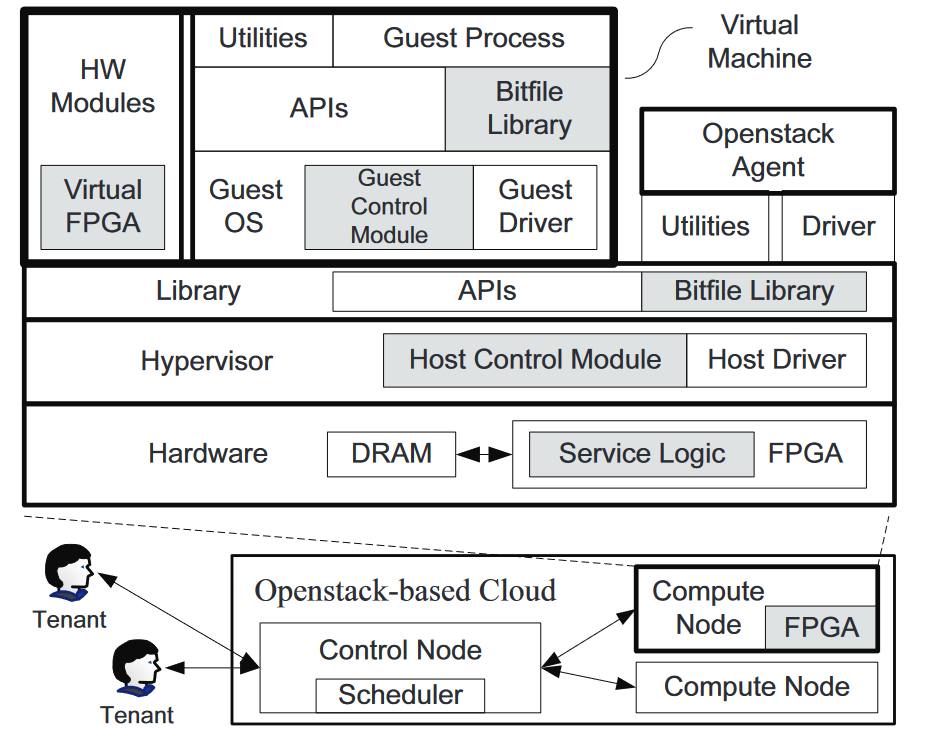
\includegraphics[width=0.8\textwidth]{chen_enabling_architecture.png}
    \caption[Cloud FPGA Architecture]{Cloud FPGA Architecture \cite{chen_enabling_2014}.}
    \label{fig:chen_enabling_architecture}
\end{figure}



\section{Cloud FPGA Security}\label{sec:cloudFPGASecurity}
Two recent works, \cite{jin_security_2020} and \cite{turan_trust_2020} have conducted comprehensive surveys of the state security in cloud based FPGAs. In \cite{jin_security_2020}, the authors discuss several avenues by which multi-tenant FPGAs present new vulnerabilities for FPGA compromise. Additionally, they present a number of solutions for access control in a multi-tenant environment. One such suggestion is the inclusion of a Secure Authentication Module (SAM), which enables verification of each IP by means of a challenge-response protocol. The work does not go into detail about this implementation, but one potential for SAM implementation is Xilinx and Silex Insight's Hardware Security Module (HSM), which facilitates secure key storage and management, as well as a cryptographic engine that could be harnessed for the secure key storage.

The authors of \cite{jin_security_2020} also discuss efforts investigating a novel method of mitigating the other primary concern of a co-tenant FPGA: side channel attacks. As the presence of malicious tenants fully under their own control (as opposed to reliant on an obscured trigger) poses a much higher threat, additional safeguards are needed to limit the amount of information that can be gained from the traditional side channels. One key vulnerability they focus on is power draw. To mitigate the extraction of data through the power side channel, they discuss research that proposes actively injecting noise into power traces, as well as attempting to actively adjust power draw to produce a constant consumption rate regardless of the needs of the functional logic.

The authors of \cite{turan_trust_2020} similarly surveys a wide body of research in the area of cloud computing. One particularly noteworthy idea they present is a research effort that attempts to provide authenticity to a bitstream by associating it with an accompanying software application, which runs on the CPU. In this model, the secure software is responsible for decrypting and programming the bitstream, providing the opportunity for suppliers to ensure that the bitstream is not compromised.

Similar to the efforts discussed previously in this section, \cite{turan_trust_2020} also presents an effort to facilitate the secure implementation of Multi-Tenant FPGAs. Specifically, they discuss an effort wherein a specific FPGA can be provided from a trusted vendor with a pair of asymmetric keys pre-configured, such that the integrator can provide the public key to IP providers to encrypt their bitstreams. In this way, no substantial storage overhead or complex key negotiation effort is required at the time of reconfiguration.

\section{Multi-Tenant Cloud Based FPGA Implementation in Literature}\label{sec:LitImpl}
In ``Cryptographically Secure Multi-Tenant Provisioning of FPGAs''\cite{bag_cryptographically_2020} Bag et al. outline a comprehensive architecture for the implementation of a cloud-compatible FPGA architecture, from which much of the work undertaken by this research effort is derived. This work proposes a platform wherein multiple discrete tenants can occupy VFPGA partitions of a larger PFPGA device in a secured environment. In their proposal, they utilize Key Aggregation Cryptography (KAC) to facilitate the encryption of a symmetric (AES) key, which in turn can be used to decrypt tenant bitstreams within their allocated partition. In this implementation, they utilize a single KAC decryption engine at the PFPGA level, which extracts the AES key and furnishes it to individual AES engines at the VFPGA level. The authors claim that by implementing their design in this manner, the only party which the tenant is required to trust is the FPGA Vendor, who provides the public and private keys used by the KAC engine to decrypt the symmetric key. It should be noted that this work is an extension of \cite{chen_enabling_2014}, discussed previously in Section \ref{sec:fpgaCloud}.


\subsection{Implementation Evaluation}\label{subsec:LitEval}
However, this claim is not completely true. By virtue of decrypting the symmetric key at the PFPGA layer, the Cloud Service Provider (CSP) is in possession of both the encrypted bitstream and the symmetric key required to decrypt it. In essence, this is equivalent to them having access to the IP contained within the bitstream itself. Therefore, the tenant must necessarily also trust the CSP, which is not a policy compatible with the security needs of many would-be tenants.Furthermore, the decrypted AES key is stored into memory, which must be isolated. Unfortunately, resolving this concern by isolating this data from the greater PL is not feasible, as there can be only one entry point into the PL from the DDR, which must be shared with all users. However, if trust can be extended to the static partition (through, say, an FPGA Vendor or third-party certified) bitstream, then DMA isolation units can be employed within each partition to prevent malicious access to the decrypted AES key and the bitstream content. This concept is explored in detail later in this work.

Additionally, this implementation allocates a considerable amount of resources to the multiple identical AES decryption cores, which don't actually yield any additional security benefit since the AES key is present at the PFPGA layer alongside the bitstream it encrypts. Furthermore, this implementation requires a predefined number of VFPGAs per PFPGA, which constrains the CSP's ability to adjust the size and number (inversely) of VFPGAs per PFPGA to adapt to demand. This is a significant limitation for CSPs as the field grows, as flexibility in trading VFPGA size for instance count could be highly advantageous in a volatile tenancy environment. This concept also forms one of the key tenants of this research effort, and is explored in great detail in the remainder of this work.